\documentclass[preprint2,numberedappendix,tighten,twocolappendix]{aastex6}  % USE THIS TO MAKE BIB, THEN FORMAT USING EMULATEAPJ
%\documentclass[twocolumn,apj,numberedappendix]{emulateapj}
\shorttitle{Epoch of Reionization Power Spectrum Results from PAPER-128}
\shortauthors{Cheng et al.}

\usepackage{amsmath}
\usepackage{graphicx}
\usepackage[figuresright]{rotating}
\usepackage{natbib}
\usepackage{ctable}
\citestyle{aa}

%		Math Shortcuts from Adrian
%\def\b{\mathbf{b}}
%\def\k{\mathbf{k}}
%\def\r{\mathbf{r}}
%\def\q{\mathbf{q}}
%\def\b{\mathbf{b}}
%\def\kp{\mathbf{k}^\prime}
%\def\kpp{\mathbf{k}^{\prime\prime}}
%\def\V{\mathbb{V}}
%\def\At{\tilde{A}}
%\def\Vt{\tilde{V}}
%\def\Tt{\tilde{T}}
%\def\tb{\langle T_b\rangle}
%\newcommand{\vis}{\mathbf{v}}
%\newcommand{\x}{\mathbf{x}}
%\newcommand{\xhat}{\hat{\mathbf{x}}}
%\newcommand{\nhat}{\hat{\mathbf{n}}}
%\newcommand{\A}{\mathbf{A}}
%\newcommand{\N}{\mathbf{N}}
%\newcommand{\rhat}{\hat{\mathbf{r}}}
%\newcommand{\khat}{\hat{\mathbf{k}}}
%\newcommand{\btheta}{\boldsymbol \theta}

\newcommand{\cc}[1]{{\color{purple} \textbf{[#1]}}}

\begin{document}
\title{Epoch of Reionization Power Spectrum Results from PAPER-128}

\author{
Carina Cheng\altaffilmark{1},
et al.
}


%		Notes	
	
%Reference section with: \ref{sec:Intro}
%Reference equation with: \eqref{eq:eqtest}
%Reference figure with: \ref{fig:figtest}
%Cite paper inside sentence: \citet{ref}
%Cite paper at end of sentence: \citep{ref}
%Cite paper inside a parenthetical sentence: \citealt{ref}

%To compile with references shown, compile in BibTeX once and LaTeX twice


%		Sample Equation Syntax
%\begin{equation}
%\label{eqtest}
%\langle \widetilde{T} (\mathbf{k}) \widetilde{T}^* (\mathbf{k^\prime}) \rangle = (2 \pi)^3 \delta^D (\mathbf{k} - \mathbf{k}^\prime) P(k),
%\end{equation}


\altaffiltext{1}{Astronomy Dept., U. California, Berkeley, CA}
%\altaffiltext{2}{Hubble Fellow}
%\altaffiltext{2}{Radio Astronomy Lab., U. California, Berkeley, CA}
%\altaffiltext{3}{Berkeley Center for Cosmological Physics, Berkeley, CA}
%\altaffiltext{3}{Dept. of Physics and Astronomy, U. Pennsylvania, Philadelphia, PA}
%\altaffiltext{8}{School of Earth and Space Exploration, Arizona State U., Tempe, AZ}

\begin{abstract}
\end{abstract}


\section{Introduction}
\label{sec:Intro}

\cc{Need to cite papers...}

The Epoch of Reionization (EoR) represents an uncharted phase in cosmic history when the first stars and galaxies ionized the neutral hydrogen present in the early Universe. During this time, it is believed that baryonic matter fell into dark matter potential wells, gravitationally collapsing into the first luminous structures. These sources, possibly quasars or young dwarf galaxies, emit radiation that ionized the abundant hydrogen in the intergalactic medium (IGM). The subsequent formation of a web of galaxies across an ionized IGM is thought to represent the large scale structure that we observe today.

The EoR has not yet been directly detected. However, constraints have been made on its timing and duration through different methods. As reionization progressed, the number of free electrons susceptible to Thompson scattering increased, resulting in scattered cosmic microwave background (CMB) photons whose imprint has been left on CMB observations. In particular, the Thompson scattering optical depth parameter $\tau$ is a useful metric for characterizing the duration of reionization. Recent \textit{Planck} measurements of $\tau$ suggest a late reionization history, occurring between redshifts of $7.7$ and $8.7$.

Galaxy observations have also begun to place constraints on the EoR. With their high luminosities, quasars make for powerful probes of the state of the IGM through absorption line studies. As photons from a quasar are redshifted, they may be absorbed by neutral hydrogen at the Lyman-$\alpha$ line, producing Gunn-Peterson trough features in quasar spectra. Observations of these spectra in high redshift galaxies have signalled the end of reionization by $z ~ 6$, and experiments are continuously pushing galaxy observations to higher redshifts. 

A third powerful probe of the EoR makes use of the 21\,cm wavelength emission produced by hydrogen due to its two quantum states. Because hydrogen is so pervasive in the Universe and a transition from its spin up state to spin down state gives off a  well-defined energy difference in the form of a 21\,cm wavelength photon, observations targeting this signal have the potential to trace the EoR from start to finish. However, 21\,cm experiments face major challenges, including those from bright foregrounds and instrumental systematics. Nevertheless, the observations and analyses of data from current radio telescope arrays have already begun to constrain the 21\,cm signal and make statements about the nature of the IGM during the EoR. 

Major existing 21\,cm experiments include both those targeting to measure the sky-averaged `global' 21\,cm signal and those employing interferometric elements and the use of cross-correlations and statistical power-spectral measurements. Examples of the former are EDGES, the LWA, LEDA, DARE, BIGHORNS, and SARAS. Major interferometers include the GMRT, LOFAR, the MWA, the 21CMA, and PAPER.

In this paper we present results from the $128$ antenna configuration of the Donald C. Baker Precision Array for Probing the Epoch of Reionization (PAPER). PAPER is a highly redundant array consisting of dual-polarization dipole antennas. Its configuration is optimal for boosting power spectrum sensitivity and the analysis used relies on a foreground avoidance approach where we measure power spectrum values in a region of delay space that is uncontaminated by foregrounds. Previous upper limits on the EoR power spectrum include those made by PAPER-32, which used its redundant configuration to its advantage to obtain an upper limit of $\Delta^{2}(k) \leq (41 {\rm mK})^{2}$ at $k=0.28h {\rm Mpc}^{-2}$. Doubling in array size and employing an updated analysis pipeline that included fringe-rate filtering and an optimal quadratic estimator framework for the power spectrum analysis achieved an upper limit on $\Delta^{2}(k)$ of $(22.4 {\rm mK}))^{2}$ in the range $0.15 < k < 0.5h {\rm Mpc}^{-1}$ at $z = 8.4$. The result from PAPER-64 was the best published upper limit thus far, with PAPER-128 achieving a factor of ?? in improvement.

PAPER-128 has been able to use much of the same technical analysis framework from previous PAPER analyses, while improving on the limits set by PAPER-64 with a longer observing time, double the number of antennas, and the development of new data quality tests, signal loss simulations, and inverse covariance weighting techniques. 

The organization of the paper is as follows. ...

\section{Observations}
\label{sec:Obs}

\begin{figure*}[!]
	\centering
	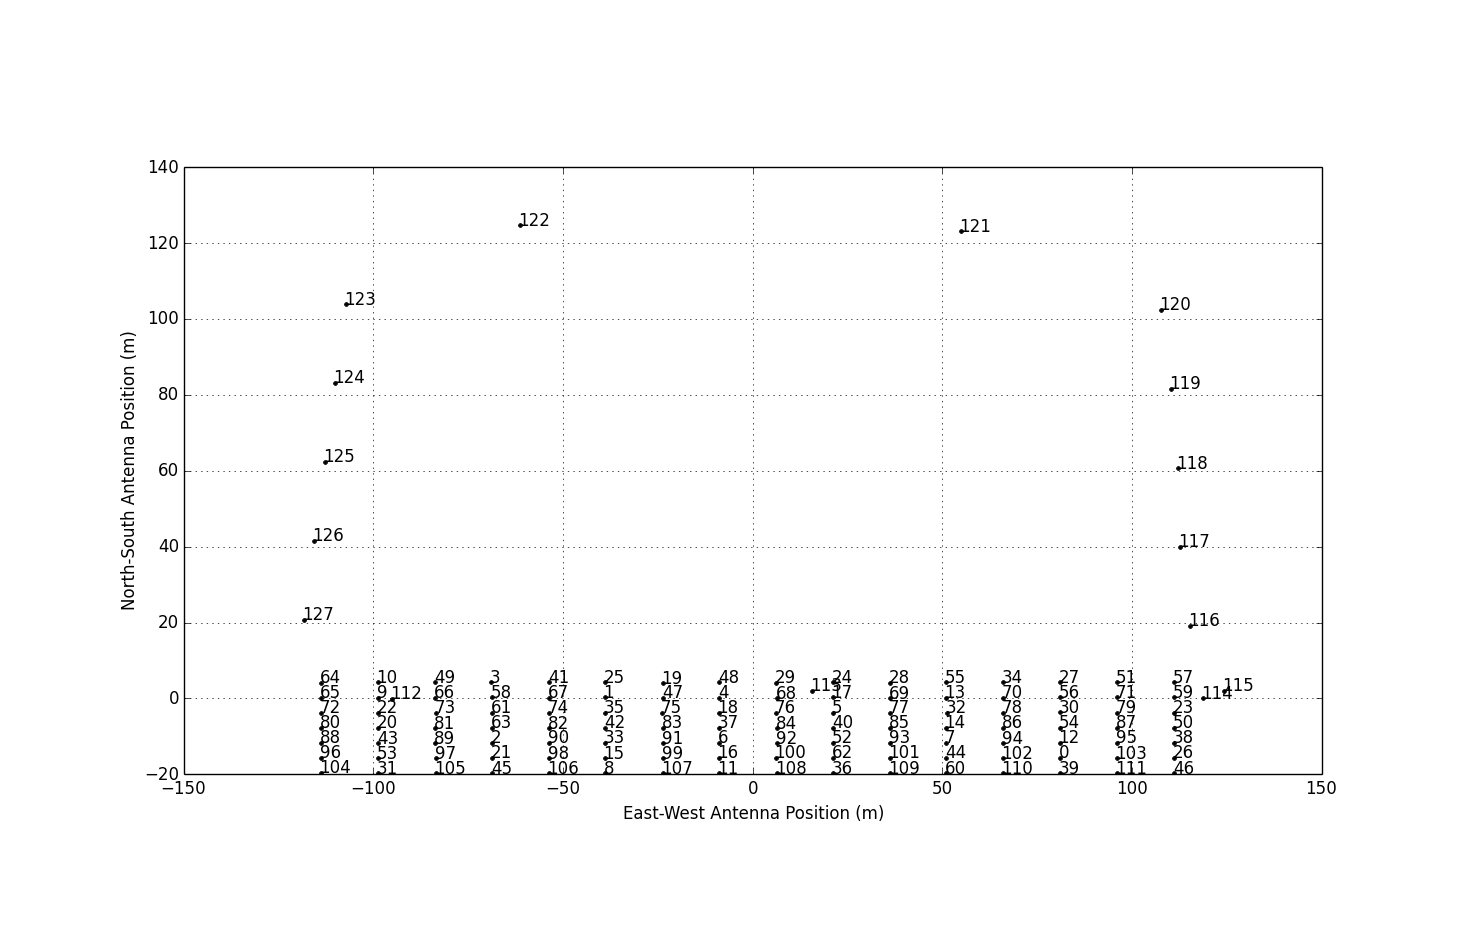
\includegraphics[width=1.0\textwidth]{antlayout.png}
	\caption{The antenna layout of PAPER-128. Core grid antennas are labeled $1$ through $111$ and outrigger antennas are labelled $112$ through $127$.}
	\label{fig:layout}
\end{figure*}

PAPER is located in the Karoo desert in South Africa at a latitude of $-30:43:18$ and longitude of $21:25:42$. The PAPER-128 antenna configuration is shown in \ref{fig:layout}. It consists of a $7$x$16$ core grid of antennas and $16$ outrigger antennas, some of which are located inside the core grid and some placed farther away to establish longer baselines. The analysis carried out in this paper makes use of only the core grid of antennas, with the East-West direction shown in \ref{fig:layout} as to the right and left. Adjacent East-West baselines have a length of $15 m$ and adjacent North-South baselines have a length of $4 m$. The baselines used in our analysis are...

The PAPER signal chain consists of drift-scan antenna elements...
The PAPER beam is...

The PAPER-128 observing season began in November, 2013, with nightly data taken for approximately $4$ months. The second observing season started up again in June, 2014 and lasted until February, 2015. Both these seasons encompass part or all of the months corresponding to our optimal observing season for which the Galaxy is below the horizon. Collectively, PAPER-128 logged $233$ nights of raw data. In this analysis, we use $??$ nights of data from season $??$. We exclude nights of known hardware malfunctioning (power failures, overheating of equipment, etc.), as well as outlier nights whose data did not pass our quality checks (see: quality paper). For our analysis, we use an LST range of $??$ which corresponds to observations of a `cold patch' of the night sky. All polarization products are saved, but we only make use of the XX and YY polarizations in this paper.

\section{Data Reduction}
\label{sec:Cal}

Raw PAPER data consists of $1024$ frequency channels sampled every $97.6 {\rm kHz}$. Every $10$ minute file then goes through our compression pipeline, which consists of a two-step radio frequency interference (RFI) flagger and averaging along both the frequency (delay filtering) and time (fringe rate filtering) axes. Final compressed data consists of $203$ frequency channels covering a bandwidth of $100-200 {\rm MHz}$. Each $10$ minute file contains data sampled at integrations of $31.65 {\rm s}$. The amplitudes of one night of raw and compressed data is shown in \ref{fig:raw} as waterfall plots of frequency versus time. 

\begin{figure*}[!]
	\centering
	%\includegraphics[width=1.0\textwidth]{raw.png}
	\caption{Waterfall plots (in log Jy) of one night of raw PAPER-128 data (left) and the same data after compression (right). Compression downsizes files by averaging over time and frequency and flags radio frequency interference.}
	\label{fig:raw}
\end{figure*}

\subsection{Redundant Calibration}

The sought-after 21\,cm signal lies beneath bright foregrounds and various instrumental systematics that contaminate our data. Because foregrounds are predicted to be $4-5$ orders of magnitude brighter than the cosmological signal, 21\,cm experiments require high dynamic ranges and considerable sensitivities. PAPER is designed to boost its sensitivity by containing many short, repeated baselines of the same length and orientation in its array. Thus, PAPER is able to measure the same Fourier-mode on the sky multiple times while beating down the amount of noise with each successive measurement.

Calibration of antennas in a redundant array is therefore crucial in order to maximize sensitivity. In our raw data, visibility measurements from two identical baseline types are not necessarily equal. This is due to changing system temperatures and different signal chains as data flows from each antenna into the correlator. However, PAPER's redundant layout can be used to solve for complex antenna gains, which when applied to the data, bring all visibility measurements for a specific baseline type into alignment. 

Redundant calibration has proven to be a powerful tool. PAPER-64 relied on redundant calibration to achieve its power spectrum limits, and here we update our method and tools and apply it to PAPER-128. As a review, let's start with the visibility measurement equation:

\begin{eqnarray}
\label{eq:viseq}
V_{ij}' &=& g_{i}^{*}g_{j}V_{ij} + n_{ij} \\
g_{j} &=&\eta_{j} + i\phi_{j}
\end{eqnarray}

Here $V_{ij}'$ represents a measured visibility for a baseline with antennas $i$ and $j$, $V_{ij}$ represents the `true' sky visibility for that same baseline, $g_{i}$ and $g_{j}$ are the complex gain factors for each antenna, and $n_{ij}$ is noise. Each gain number consists of an amplitude $\eta$ and phase $\phi$. The visibility equation can be written down for all baselines and - without using array redundancy - would not be least squares solvable because the number of unknowns ($2N+N(N-1)/2$) is greater than the number of measurements ($N(N-1)/2$), where $N$ is the number of antennas . However, if $V_{ij}$, the `true', or `model' visibility, is constrained to be the same for all identical baselines, the system of equations becomes solvable.

For our analysis, we use the package {\sc Omnical} for redundant calibration. Similarly to the analysis of PAPER-64, {\sc Omnical} comprises of three steps. The first is {\tt FirstCal}, which uses all baseline redundancies to generate a static gain solution for each antenna that will unwrap any phase wrapping between two identical baselines. We perform {\tt FirstCal} because the next stage of {\sc Omnical} cannot tell the difference between a phase of $0$ and $2\pi$, for example. The second step is {\tt LogCal}, which takes the log of all the visibility equations and separates the real and imaginary components into two matrices. Coarse solutions are determined for both the antenna gains and `model' visibilities (one for each baseline type) simultaneously. The final step of {\sc Omnical} is {\tt LinCal},, which applies small perturbations to the {\tt LogCal}, solutions in an iterative fashion, honing in on the optimal solutions.

We perform redundant calibration for each epoch of data used in our analysis, as each epoch has to be separately calibrated since they are on different overall gain scales. We divide out the antenna gains for each of our measured visibilities, bringing them into alignment with each other (for identical baseline types) and the `model' visibility for that baseline type. We also include the subtraction of crosstalk in our dataset. Crosstalk shows up as a constant signal in time in our visibilities and is attributed to signals from one antenna being picked up by another. {\sc Omnical} handles crosstalk by subtracting off an averaged residual (differences between measured visibilities and the `model' visibility, averaged over baseline type) for each visibility measurement.

For PAPER-128, we update the {\sc Omnical} software package, originally written in C, with a user-friendly interface written in Python.  Additionally, we employ a chi-square metric on a per antenna basis in order to exclude dead or faulty antennas and improve our calibration solutions. \cc{Add plots to show stability of {\sc Omnical} solutions and chi-square examples}
 
It is important to note that while {\sc Omnical} is powerful for ensuring array redundancy, it is not able to solve for $4$ calibration parameters - namely, to correct for the overall gain, phase, and tip/tilt of the array. In order to do this, we turn to...

\subsection{Bandpass Calibration}

\subsection{Delay-Domain Foreground Removal}

Foregrounds pose a significant challenge to EoR experiments. Some experiments, like LOFAR and the MWA, rely on modelling and foreground subtraction to create a clean EoR `window' in which to make their power spectrum measurements. Previous PAPER results, including this one, instead focus on a foreground avoidance approach. 

In order to filter foregrounds, we exploit their spectrally-smooth nature. By Fourier-transforming our visibilities along the frequency axis, the delay domain provides a natural space in which to isolate foregrounds. Physically, a time delay can be thought of as the extra time light from a source takes to reach one antenna compared to another one (due to slightly different travelling distances). The maximum delay a source on the sky can have is if it is located on the horizon. In this case, the delay is determined by the length of the baseline. Consequently, all spectrally-smooth foreground signals show up within a maximum delay (or `horizon limit') given a baseline length. The EoR signal, however, is believed to mimic noise which has a random frequency structure and is not confined to be within the horizon limit. A simple way to avoid foregrounds without removing the cosmological signal, therefore, is to make our power spectrum measurements outside of the horizon limit that contains the bright foregrounds. 

In practice, we filter our calibrated visibilities by de-convolving out our sampling function (which contains flags due to RFI) from our delay-domain visibilities using a CLEAN-like algorithm and restricting our clean components to inside the horizon limit (set by the baseline length) plus a $15 {\rm ns}$ buffer. The Fourier-transformed clean components are then subtracted from our visibilities. This filtering process is performed on a per-baseline, per-integration basis, and we achieve a brightness suppression of $~2$ orders of magnitude in our visibilities. 

\subsection{RFI Removal, LST-Binning, and Absolute Calibration}

We perform a final round of RFI-removal by flagging visibilities that lie more than $4\sigma$ above the mean on a time, frequency, and baseline basis. \cc{we flag specific channels before delay filtering too, to avoid leakage outside of the horizon limit due to Fourier-transforming super un-smooth signals}

Finally, we stack our data in LST into two datasets, alternating between even and odd Julian Dates to create an `even' and `odd' LST-binned dataset. \cc{other jack-knife tests...}

Recalling that redundant calibration through {\sc Omnical} does not solve for the overall calibration parameters of our array, we calibrate these final unknowns by matching our LST-binned datasets with that of PAPER-64. For the PAPER-64 analysis, absolute calibration was carried out by standard radio astronomy self-calibration. Overall phase terms were fitted using Pictor A, Fornax A, and the Crab Nebula, and the overall flux scale was determined using Pictor A as a calibrator source. PAPER-64's analysis produced even and odd LST-binned data covering an LST range of $0-8$, fully encompassing the LST ranges we use in our analysis. 

We match the overall gain scale of our data to that of PAPER-64 by fitting an 8th order polynomial to the time-averaged ratio of the two LST-aligned foreground-containing datasets and then applying that polynomial to our foreground-filtered LST-binned datasets. Similarly, we match the overall phase by fitting a linear line to the phase difference between PAPER-128 and PAPER-64. 

\subsection{Fringe-Rate Filtering}

In order to further suppress foregrounds and instrumental noise, we weight our visibilities on a temporal basis in a technique known as fringe-rate filtering. We take the Fourier transform along time to enter fringe-rate space, in which our data spans a range of fringe-rates determined by our integration time. In the fringe-rate domain, it is a natural space in which to filter out noise that is not associated with the rotating sky. This is because signals attached to the sky have a maximum fringe-rate set by the rotation velocity of the Earth (i.e. sources at the equator appear the move the fastest), and therefore any signals that exceed this fringe-rate cannot be the cosmological signal and can safely be filtered without any loss of information. 

It was shown in \citet{parsons_et_al2016} that filtering in fringe-rate space is equivalent to weighting data by the primary beam. Because of this, we determine an optimal fringe-rate filter that up-weights parts of the sky that our beam is most sensitive to, while down-weighting the opposite. We also filter out the zero fringe-rate bin, which contains signals that are constant in time, such as crosstalk. We then apply the filter on a per-baseline basis as a convolution in the time-domain, which has the affect of averaging our data in time. 

Using an optimal fringe-rate filter comes at the cost of signal loss due to a reduction of the number of independent time samples in our dataset...

\section{Power Spectrum Analysis}
\label{sec:PS}

With our final visibilities in hand, we are ready to estimate the 21\,cm power spectrum, $\hat{\textbf{p}}(\textbf{k})$. The power spectrum measurement is a function of $\textbf{k} = (k_{x},k_{y},k_{z})$, where each component of $k$ represents the Fourier-dual to spatial coordinates $(x,y,z)$. Our visibilities have already been Fourier-transformed along two of these axes, namely, along $k_{\perp} = \sqrt{k_{x}^{2}+k_{y}^{2}}$. This perpendicular component of $k$ is analogous to the spatial Fourier-modes in the plane of the sky, while the parallel component of $k$, $k_{\parallel}$, is the Fourier-transform of our visibilities along the line-of-sight (in the frequency direction). 

Our visibilities measure the sky temperature in units of Jys. Recalling that we are interested in the power of the cosmological signal on different $k$-scales, we can map our data to a power spectral measurement using the standard definition

\begin{equation}
\label{eq:ps}
\langle \tilde{T}_{b}(\textbf{k})^{*}\tilde{T}_{b}(\textbf{k'})\rangle = (2\pi)^{3} \delta^{D}(\textbf{k}-\textbf{k'})\hat{\textbf{p}}(\textbf{k})
\end{equation}

\noindent where $\tilde{T}_{b}(\textbf{k})$ is the spatial Fourier-transform of the brightness temperature of the sky, $\delta^{D}$ is the Dirac delta function, and $\langle \rangle$ is an ensemble average. As a simplistic explanation, we need to take our visibility temperature measurements, Fourier-transform them along the frequency axis and convert from units of Jys to Kelvin, square, and bin in constant contours of $k$. In practice, however, we use linear algebra techniques as explained in the following section in order to obtain both $\hat{\textbf{p}}(\textbf{k})$ and its associated error bars. 

\subsection{Optimal Quadratic Estimators}
\label{sec:OQE}

We follow the optimal quadratic estimator (OQE) formalism used by \citet{ali_et_al2015} to form estimates of our power spectrum $\hat{\textbf{p}}(\textbf{k})$. As a brief review, we recap the method here as applied to our data. 

We begin with the data vector $\textbf{x}$, which consists of our visibility measurements as a function of time and frequency for each baseline. We divide our data into separate datasets by baseline type, and apply the OQE formalism to each separately, forming multiple power spectra. In our analysis, we use \cc{??} types of baselines. After forming the power spectra, we fold them into our final power spectrum by \cc{??}.

Recalling that our goal is to measure power spectrum values as a function of \textbf{k}, the Fourier dual to the spatial directions, the next step is to form the set $\hat{q}_{\alpha}$. This quantity, defined as  

\begin{equation}
\label{eq:qhat}
\hat{q}_{\alpha} = \frac{1}{2}\textbf{x}^{\dagger}\textbf{C}^{-1}\textbf{Q}_{\alpha}\textbf{C}^{-1}\textbf{x}-b_{\alpha}
\end{equation}

\noindent represents power spectrum quantities (un-normalized) for each $k$ bin indexed by $\alpha$. Here we see two copies of our data vector \textbf{x} and two copies of $\textbf{C}^{-1}$ where $\bf{C} \equiv \langle\textbf{x}\textbf{x}^{\dagger}\rangle$, the true covariance matrix of \textbf{x}. The operator $\textbf{Q}_{\alpha}$ transforms our visibilities into power spectrum space by performing a Fourier transform along the frequency axis, and $b_{\alpha}$ is a noise bias that is subtracted off.

In practice, $\bf{x}$ has dimensions of time versus frequency and exists for every baseline (in a given redundant group), and group (such as an `even' or `odd' LST-binned set). Notice that there is a copy of $\textbf{C}^{-1}\textbf{x}$ on each side of the expression for $\hat{q}_{\alpha}$. When performing this computation, we do not allow the cross-multiplication to occur if both quantities are derived for the same baseline, or the same group. For example, we do not allow $(\textbf{C}^{-1}\textbf{x})_{even'A}$ to be multiplied with $(\textbf{C}^{-1}\textbf{x})_{even,B}$ since both quantities are formed from the `even' dataset, nor do we allow $(\textbf{C}^{-1}\textbf{x})_{even,A}$ to be multiplied with $(\textbf{C}^{-1}\textbf{x})_{odd,A}$, since both quantities are formed for baseline $A$. We do not include these cases in order to eliminate any biases from allowing auto power from identical baselines or groups to remain.

For faster computation (due to less cross-multiplications), we divide our baselines into $5$ subgroups and sum up the quantities $\textbf{C}^{-1}\textbf{x}$ for each. We still do not allow $\hat{q}_{\alpha}$ to be computed if the same baseline appears in both subgroups that are being cross-multiplied. 

Once we have formed our $\hat{q}_{\alpha}$s, we can normalize them using the matrix \textbf{M}. Namely,

\begin{eqnarray}
\hat{\textbf{p}} = \textbf{M}\hat{\textbf{q}}
\end{eqnarray}

\noindent where $\hat{\textbf{p}}$ is the normalized estimate of the true power spectrum $\textbf{p}$. Before we compute \textbf{M}, we define the Fisher matrix \textbf{F} to be

\begin{eqnarray}
\textbf{F}_{\alpha\beta} = \frac{1}{2}tr(\textbf{C}^{-1}\textbf{Q}_{\alpha}\textbf{C}^{-1}\textbf{Q}_{\beta})
\end{eqnarray}

\noindent where $\alpha$ and $\beta$ represent different bandpowers or $k$ bins. The Fisher matrix encodes information about \cc{??}. It is related to the normalization matrix \textbf{M} by the window function matrix \textbf{W}, which relates the true power spectrum \textbf{p} with our estimates $\hat{\textbf{p}}$:

\begin{eqnarray}
\textbf{W} &=& \textbf{MF} \\
\hat{\textbf{p}} &=& \textbf{Wp}
\end{eqnarray}

\noindent The window function is constructed so that each row sums to unity. This ensures proper normalization of the power spectrum estimates. In practice, we have a choice of \textbf{M} and in our analysis choose to use a method where it is determined from the Cholesky decomposition of \textbf{F}... \cc{this may change...}. 

\subsection{Signal Loss}
\label{sec:Sigloss}

Both the fringe-rate filtering and inverse covariance weighting of our visibilities produces data that is susceptible to signal loss. This is due to the reduction of independent time samples from fringe-rate filtering which leads to a more noisy dataset. Consequently, when computing $\textbf{C}^{-1}$ from the data, the result from the inverse covariance weighting of that same data is to over-fit the noise. This can produce power spectra values below the thermal noise limit that is predicted based on observation parameters. 

We recognize that the permutation of fringe-rate filtering and then applying the OQE framework, as well as our choice for $\textbf{C}^{-1}$, play a large role in the amount of signal loss that results. In order to quantify signal loss, we run simulations where various levels of an EoR-like signal are added on top of our data. This injected signal, $\textbf{e}$, resembles the predicted EoR signal by mimicking random noise and by being common to all baselines. It is fringe-rate filtered in the same way as our data, representing what could be the cosmological signal contained within our data. We then compare the input and output power spectrum of $\textbf{e}$ as our full OQE framework is applied.

Mathematically, suppose the addition of the injected signal onto our data is

\begin{equation}
\textbf{x} + \textbf{e} = \textbf{r}.
\end{equation}

The input power spectrum of $\textbf{e}$ is computed as the power spectrum that results when an identity matrix \textbf{I} is used to replace any covariance matrices used in our pipeline. Ignoring normalization factors, this is written as

\begin{equation}
P_{in} \propto \textbf{e}^{\dagger}\textbf{I}^{-1}\textbf{Q}\textbf{I}^{-1}\textbf{e}
\end{equation}

\noindent and there is no signal loss associated with this computation. The expression for the output power spectrum, $P_{out}$, is comprised of two terms - the covariance treated power spectrum associated with \textbf{r}, and that of \textbf{x} alone. 

\begin{eqnarray}
\label{eq:sigloss}
\textbf{p}_{x} + \textbf{p}_{e} = \textbf{p}_{r} \\
P_{in} \equiv \textbf{p}_{e} &=& \textbf{p}_{r}-\textbf{p}_{x} \nonumber \\
&\propto& \textbf{r}^{\dagger}\textbf{C}_{r}^{-1}\textbf{Q}\textbf{C}_{r}^{-1}\textbf{r} - \textbf{x}^{\dagger}\textbf{C}_{x}^{-1}\textbf{Q}\textbf{C}_{x}^{-1}\textbf{x} \nonumber
\end{eqnarray}

The explicit signal loss calculation described here is new to the PAPER-128 analysis. We test the expression in \eqref{eq:sigloss} by running several simulations without data (i.e. pure noise) in order to verify its output. \cc{reference signal loss paper?}

The ratio of $P_{in}$ to $P_{out}$ changes as the level of the injected signal \textbf{e} is increased. As shown in \cc{reference figure here}, when the injected signal level is low compared to the data \textbf{x}, the recovered output power spectrum is the same as the input. However, when \textbf{e} begins to dominate over  \textbf{x}, we move to a regime where the input power spectrum is greater than the output, implying signal loss due to the over-fitting of noise during inverse covariance weighting. 

Our power spectrum for the data alone is equivalent to the second term in \eqref{eq:sigloss}, barring normalization factors. We choose to apply a conservative signal loss factor - that is, the factor that we multiply our power spectrum points by is the ratio $P_{in}/P_{out}$ that corresponds to a $P_{out}$ value equal to our highest measured power spectrum value (the point that produces the most loss). We apply this correction factor to our entire power spectrum.

\section{Results}
\label{sec:Res}

Our final 21\,cm power spectrum measurements from PAPER-128 are for a redshift of $z=\cc{??}$. The data used for this result incorporates \cc{??} days and \cc{??} channels, centered around \cc{??}. We present both the power spectrum points from $\hat{\textbf{p}}(\textbf{k})$ in units of $mk^{2}(h^{-1}Mpc)^{3}$ and the corresponding dimensionless power spectrum points, $\Delta^{2}(\textbf{k})$, which is related to $\hat{\textbf{p}}(\textbf{k})$ by

\begin{equation}
\label{eq:deltasq}
\Delta^{2}(\textbf{k}) = \frac{k^{3}}{2\pi^{2}}\hat{\textbf{p}}(\textbf{k}).
\end{equation}

\section{Conclusions}
\label{sec:Con}

\section{Acknowledgements}
\cc{NSF Graduate Research Fellowship Program (GRFP) Fellowship}
\cc{UC Berkeley Chancellor's Fellowship}
\label{sec:Ack}

\bibliographystyle{apj}
\bibliography{refs}


\end{document}

